\documentclass[a4j,twocolumn]{jsarticle}
\usepackage{amssymb} % 高度な数式を表記するために使用
\usepackage[dvipdfmx]{graphicx}		% 図を入れるときに使用
\usepackage{wrapfig}		% 図の周りに本文を流し込みたいときに使用
\usepackage{here}
\usepackage{subfigure}

\def\Vec#1{\mbox{\boldmath $#1$}}
\usepackage[dvipdfmx]{graphics}

\setlength{\textheight}{275mm}
\headheight 5mm
\topmargin -30mm
\textwidth 185mm
\oddsidemargin -15mm
\evensidemargin -15mm
\pagestyle{empty}
\begin{document}

\title{小傾角粒界エネルギーの視覚的検証を簡易化するソフト開発}
\author{関西学院大学 情報科学科 西谷研究室 1549 成田大樹}
\date{}
\maketitle

\section{はじめに}
西谷研究室では,小傾角粒界エネルギーについて,Read-Shockleyによる理論と大槻による実験結果の矛盾を解明するために様々な手法をこれまで試してきた.
両者のグラフは図\ref{fig:one}のようになり,小傾角粒界エネルギーの実験結果における相違点は,以下の通りである.
\begin{itemize}
\item Hassonらによるシミュレーション結果では,
0度,及び90度における立ち上がりの傾きがそれぞれ異なる傾きになった.

\item 大槻のシミュレーション結果では,
0度,及び90度の傾きが左右対称になった.
\end{itemize}

この矛盾を解明するために,
本研究では,
原子の配置や粒界エネルギーの高低差を視覚的に検証し易くするためのソフトを開発する.

\begin{figure}[h]
\begin{center}
\begin{tabular}{cc}
   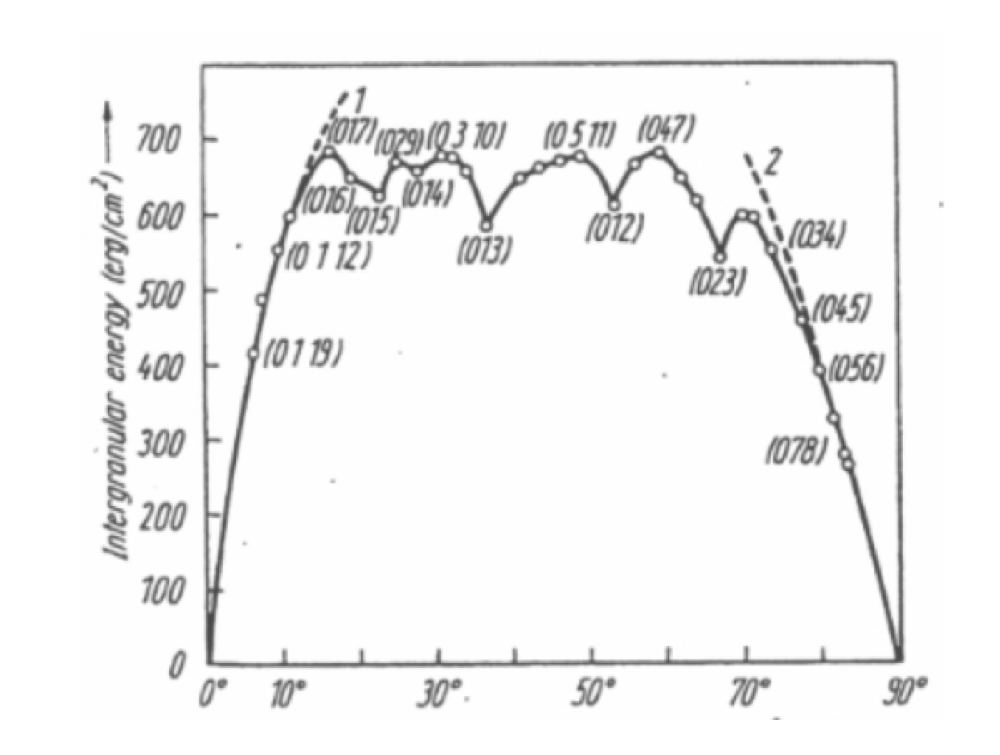
\includegraphics[width=40mm]{./Hasson.png} &
   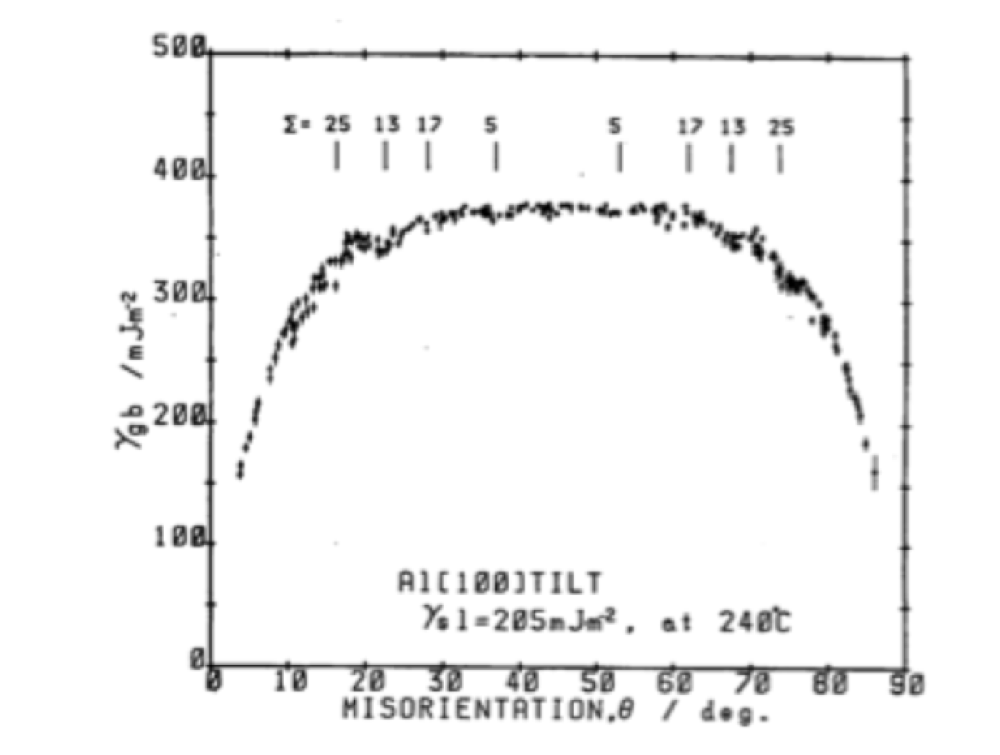
\includegraphics[width=40mm]{./Otsuki.png} \\
   (a) & (b)
\end{tabular}
  \caption{(a) Hassonと(b)大槻の求めたAl(100)対称傾角粒界エネルギーの方位依存性.}
  \label{fig:one}
\end{center}
\end{figure}

\vskip 1.5em%

\section{現状}
上記の実験結果の相違を明らかにするために,
第一原理計算ソフトVASPや原子間ポテンシャルを使ったシミュレーションをはじめ,
Sutton Vitekによる粒子モデルの研究を取り組んできた.

経験的原子間ポテンシャルによるシミュレーションをおこなった八幡の研究では,
Read-Shockleyの理論予測と同様の結果となった\cite{yahata}.

一方,岩佐の研究では,最安定な原子配置を探索するために原子の削除操作を取り入れ,
第一原理計算ソフトVASPを用いて構造緩和し,
系全体のエネルギーを計算した.
その結果,
予測通りに小傾角粒界エネルギーが大槻の結果を再現する程度の低いエネルギーとなった\cite{iwasa}.

ところが,
安定構造の原子位置を視覚的に確認をしなかったため,
図\ref{fig:two}のように原子が全体的に傾いてしまい,
粒界がより低い角度になった状態を計算し,構造緩和に過ちが生じていた.

\begin{figure}[h]
\begin{center}
   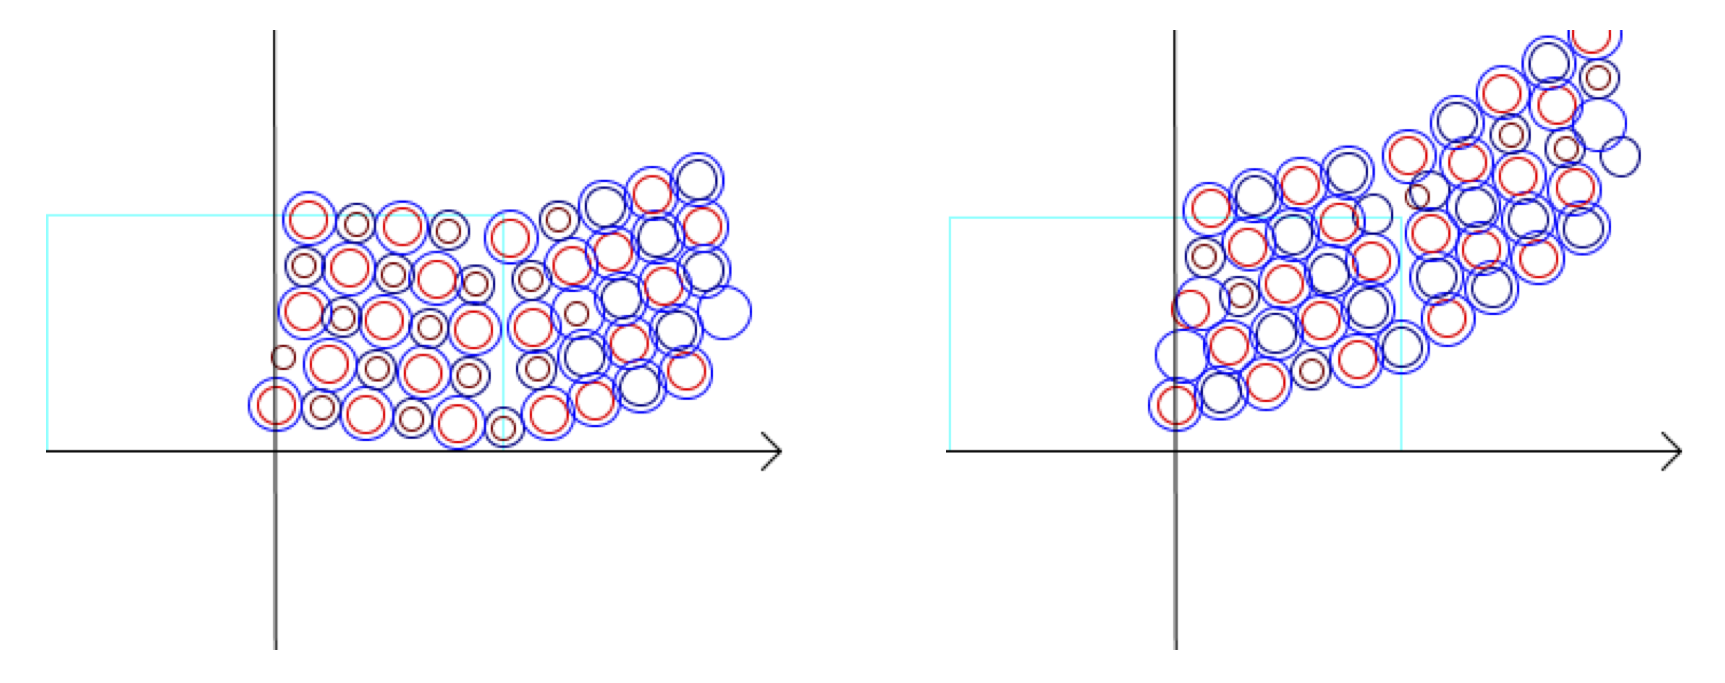
\includegraphics[width=80mm]{./Iwasa.png} 
     \caption{岩佐の研究結果.}
  \label{fig:two}
\end{center}
\end{figure}



\section{手法}
本研究のソフト開発は,MVCモデルで作成していく.
MVCモデルとは,web applicationの開発において取られている手法であり,
データ処理,画面出力,処理制御の機能が明確に分離されている.
機能の直交化により,
開発作業の分業化が容易におこなうことができ, 
処理結果を画面表示する"Viewer"の機能構築に特化した開発が可能となる.

小傾角粒界の原子モデルを視覚的に確かめるためのモデル"Viewer"は,
VASPの入出力で採用されているPOSCAR形式のファイルを入力とし,
SVGで出力する.
SVGには,以下の特徴がある.
\begin{itemize}

\item ベクトルベースで描画するため,
曲線や文字の拡大縮小しても画質が劣化することなく表示できる,

\item 汎用性が高く,画像表示や変換が容易に処理できる.
\end{itemize}

また,SVGの生成には,
Ruby言語で視覚化を容易に実現できる2次元画像描画ライブラリ"Cairo"を用いる\cite{sudoh}.

図\ref{fig:three}は,実際にSVGで描画したものである.



\begin{thebibliography}{9}
\bibitem{yahata} 小傾角粒界粒子シミュレーションの原子ポテンシャル依存性, 八幡裕也 (関西学院大学 理工学部研究科情報科学専攻 修士論文 2015).
\bibitem{iwasa} 原子削除操作を加えた対称傾角粒界のエネルギー計算, 岩佐 恭佑(西学院大学 理工学部研究科情報科 学士論文 2016). 
\bibitem{sudoh} cairo:2次元画像描画ライブラリ,須藤功平, Rubyist Magazine - るびま, Vol.54 (2016-08).
\end{thebibliography}

\end{document}
